\documentclass[ukenglish]{beamer}

%%% Dichiarazione dei pacchetti standard.
\usepackage[utf8x]{inputenc}
\usepackage{subfigure}
\usepackage{graphicx}    % inclusione graph images (eps)
\usepackage{units}
\usepackage{url}
\usepackage{lmodern}
\usepackage{booktabs}
\usepackage[T1]{fontenc}
\usepackage{import}
%gets rid of bottom navigation bars

\usetheme{Boadilla}
\usecolortheme{wolverine}

\setbeamertemplate{footline}[frame number]{}
\setbeamertemplate{navigation symbols}{} 
\graphicspath{{../../images/}}
\subimport{../../}{commands}
    
%%% Titolo e autore.
\title[Razor for Top Partners]{Razor variables in the search for Top
Partners}
\author{Matteo Abis\\
\url{matteo.abis@cern.ch}}
\institute{Università di Padova and INFN}
\date{\today}

\begin{document}

\begingroup
\setbeamertemplate{footline}{\large{\vspace*{-1cm}\centering Many thanks to the
B2G-12-003 group:\\ A.Avetisyan, P.Azzi, S.Bhattacharya, T.Bose, P.Checchia,
S.Lewin, M.Narain, M.Nespolo, S.Vanini\par}}
\begin{frame}
  \titlepage
\end{frame}
\endgroup
 
\begin{frame}
    \begin{itemize}
        \item couple to third generation
        \item solve hierarchy problem
            \begin{itemize}
                \item \emph{Contino, Servant}, JHEP 0806:026 (2008)
                \item \emph{Mrazek, Wulzer}, Phys. Rev. D81, 075006 (2010)
            \end{itemize}
        \item focus on pair production of $\mathrm{T}_{5/3}$
        \item experimental signature: same-sign leptons + jets
    \end{itemize}
    \begin{figure}[h]
        \centering
        
\includegraphics[height=.5\textheight]{toppartner_decay_top.eps}
        %\caption{Top Partners into same-sign leptons}
        %\label{fig:TTbar_feynman}
    \end{figure}
\end{frame}

\begin{frame}
    \frametitle{Top Partners}
    \begin{itemize}
        \item couple to third generation
        \item solve hierarchy problem
            \begin{itemize}
                \item \emph{Contino, Servant}, JHEP 0806:026 (2008)
                \item \emph{Mrazek, Wulzer}, Phys. Rev. D81, 075006 (2010)
            \end{itemize}
        \item focus on pair production of $\mathrm{T}_{5/3}$
        \item experimental signature: same-sign leptons + jets
    \end{itemize}
    \begin{figure}[h]
        \centering
        
\includegraphics[height=.5\textheight]{toppartner_decay_top.eps}
        %\caption{Top Partners into same-sign leptons}
        %\label{fig:TTbar_feynman}
    \end{figure}
\end{frame}

\begin{frame}
    \frametitle{Goal}
    \begin{block}
        {}
        Find new variables to reduce the main background, which is the
        data-driven \ttbar.
    \end{block}
    \alert{Very preliminary results! Focus on the method!}
\end{frame}


\begin{frame}
    \frametitle{Signal MC}
    \framesubtitle{Fall11 production}
    \subimport{../../tables/}{signal_mc}
\end{frame}

\begin{frame}
    \frametitle{Background MC}
    \framesubtitle{Summer11 production}
    \subimport{../../tables/}{background_mc}
\end{frame}

\begin{frame}
    \frametitle{Data}
    \framesubtitle{2011 golden JSON, \unit[5.0]{$fb^{-1}$}}
    \subimport{../../tables/}{data_pd}
\end{frame}

\begin{frame}
    \frametitle{Triggers}
    \subimport{../../tables/}{triggers}
\end{frame}

\begin{frame}
    \frametitle{Event cleanup}
    \framesubtitle{Standard from TLBSM recipes}
    \begin{description}
        \item[scraping]\hspace*{\fill}\\
            \begin{itemize}
                \item at least 25\% of the tracks must be high-purity for events
            with at least ten tracks
            \end{itemize}
        \item[good primary vertex] \hspace*{\fill}\\
            \begin{itemize}
                \item at least 4 degrees of freedom
                \item less than \unit[25]{cm} from interaction point in $z$
                \item less than \unit[2]{cm} radially
            \end{itemize}
        \item[HBHE noise filter] 
    \end{description}
\end{frame}

\begin{frame}
    \frametitle{Electrons}
    \framesubtitle{Standard top selection, plus charge consistency}
    \begin{itemize}
        \item $\pt > \unit[30]{GeV}$
        \item $|\eta| < 2.4$, except EBEE gap
        \item HyperTight1MC electron identification
        \item relative isolation $< 0.15$
        \item conversion rejection
        \item transverse impact parameter $< \unit[0.02]{cm}$
        \item GSF, CFT, ScPix charge consistency
    \end{itemize}
\end{frame}

\begin{frame}
    \frametitle{Muons}
    \framesubtitle{Standard top selection}
    \begin{itemize}
        \item $\pt > \unit[30]{GeV}$
        \item $|\eta| < 2.4$
        \item Global and Tracker muon
        \item relative isolation $< 0.20$
        \item $\chi^2/\text{NDF} < 10$
        \item at least one muon hit
        \item at least one pixel hit
        \item at least eleven silicon hits
        \item at least two chambers with matching segments
    \end{itemize}
\end{frame}

\begin{frame}
    \frametitle{Jets}
    \framesubtitle{Standard top selection}
    \begin{itemize}
        \item anti-$k_T$ particle flow jets
        \item $\pt > \unit[30]{GeV}$
        \item $|\eta| < 2.4$
        \item Charged hadron subtractions, L1FastJets corrections,
            L2L3 jet energy scale corrections
        \item loose particle flow identification
        \item $\Delta R(\text{lepton, jet}) > 0.3$
    \end{itemize}
\end{frame}

\begin{frame}
    \frametitle{Same-sign non-prompt background}
    \framesubtitle{Data-driven estimate, with the ``tight-loose'' method}
    \begin{itemize}
        \item details in AN-2010/261, AN-2010/257, AN-2011/258
        \item define looser lepton selection
        \item measure the probability that a lepton passing the loose
            selection also passes the tight one
        \item estimate the number of non-prompt leptons passing the tight
            selection
    \end{itemize}
\end{frame}

\begin{frame}
    \frametitle{The current selection}
    \framesubtitle{AN-11-419}
    \begin{itemize}
        \item at least four jets
        \item $H_T > \unit[300]{GeV}$
    \end{itemize}
    Thanks to the whole group of B2G-12-003, still in the approval process.
\end{frame}

\begin{frame}
    \frametitle{The razor variables}
    \framesubtitle{Rogan, \emph{Kinematical variables towards new dynamics
    at the LHC}, arXiv 1006.2727}
    \begin{block}{The standard razor}
        Two pair-produced massive particles, both decaying to a final state with
        one visible particle and \met.
    \end{block}
    \begin{block}
        {The simple version}
        \begin{align*}
            M_R &= \sqrt{(a^0 - b^0)^2 - (a^3 + b^3)^2} \\
            M_R^T &= \sqrt{\dfrac{|\vec{m}|}{2} (|\vec{a}_T| + |\vec{b}_T|) 
            -\dfrac{\vec{m}}{2} \cdot (\vec{a} + \vec{b})}\\
            R &= M_R^T / M_R
        \end{align*}
    \end{block}
    Notation:
    \begin{itemize}
        \item $a^\mu$ and $b^\mu$ are the four momenta of the visible
            particles
        \item $\vec{m}$ is the \met
        \item $\vec{v}_T$ is a vector with the transverse components
            $(v_x, v_y, 0)$
    \end{itemize}
\end{frame}

\begin{frame}
    \frametitle{Properties of the razor variables}
    \begin{description}
        \item[$M_R$] independent of a longitudinal boost, related to the
            heavy particle mass
        \item[$R$] another measurement of the scale of the process, in the transverse plane
    \end{description}

    \begin{block}
        {Additional corrections}
        The formulae in this analysis are corrected for the momentum of the
        system as a whole by boosting the vectors with the sum $\vec{a} + \vec{b} +
        \vec{m}.$
    \end{block}
\end{frame}

\begin{frame}
    \frametitle{Hadronic invariant mass}
    \framesubtitle{The easy part}
    \begin{block}{}
        Mass of the sum of the jets in the event.
    \end{block}
        \begin{figure}[h]
            \centering
            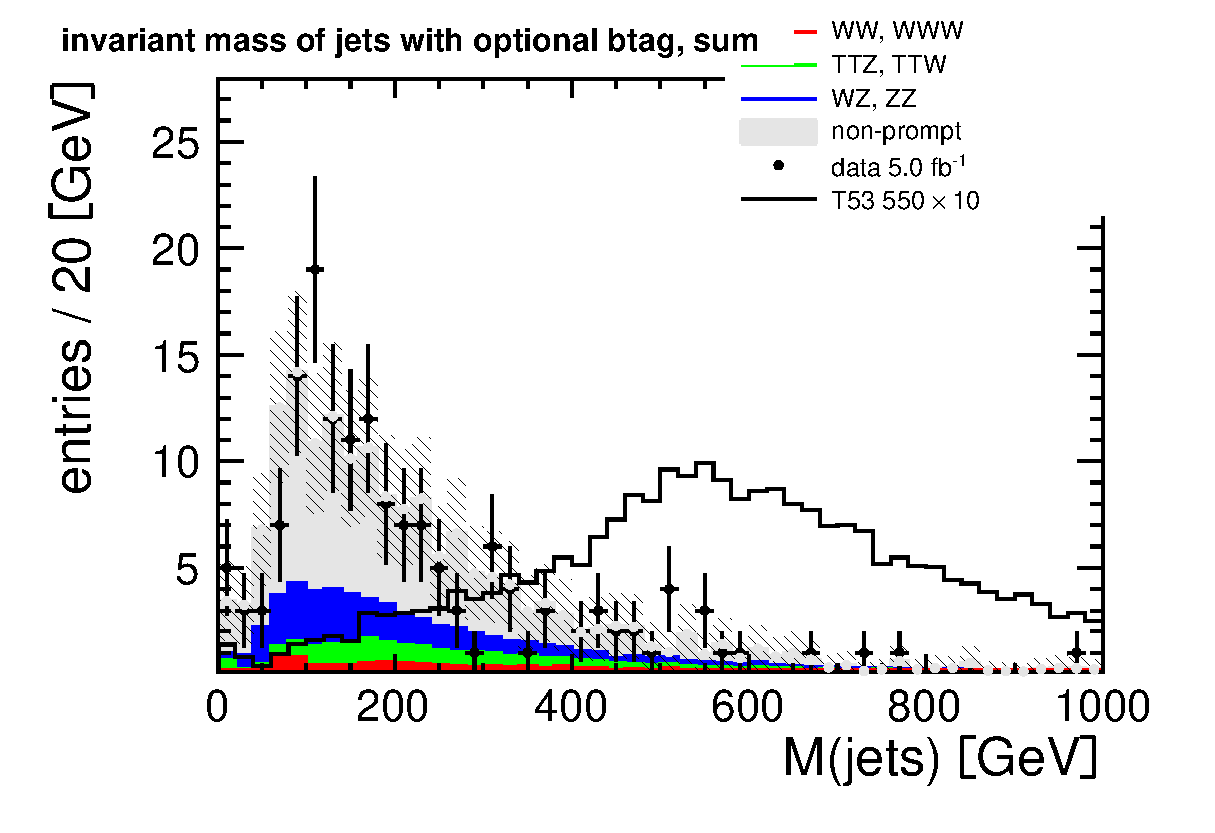
\includegraphics[width=.7\textwidth]{had_mass_optional_btag_sum.eps}
        \end{figure}
\end{frame}

\begin{frame}
    \frametitle{$M_R$}
    \framesubtitle{An indicator of the heavy particle mass scale}
    \begin{block}{}
        Peak expected around $M(\mathrm{T}_{5/3})/2$.
    \end{block}
        \begin{figure}[h]
            \centering
            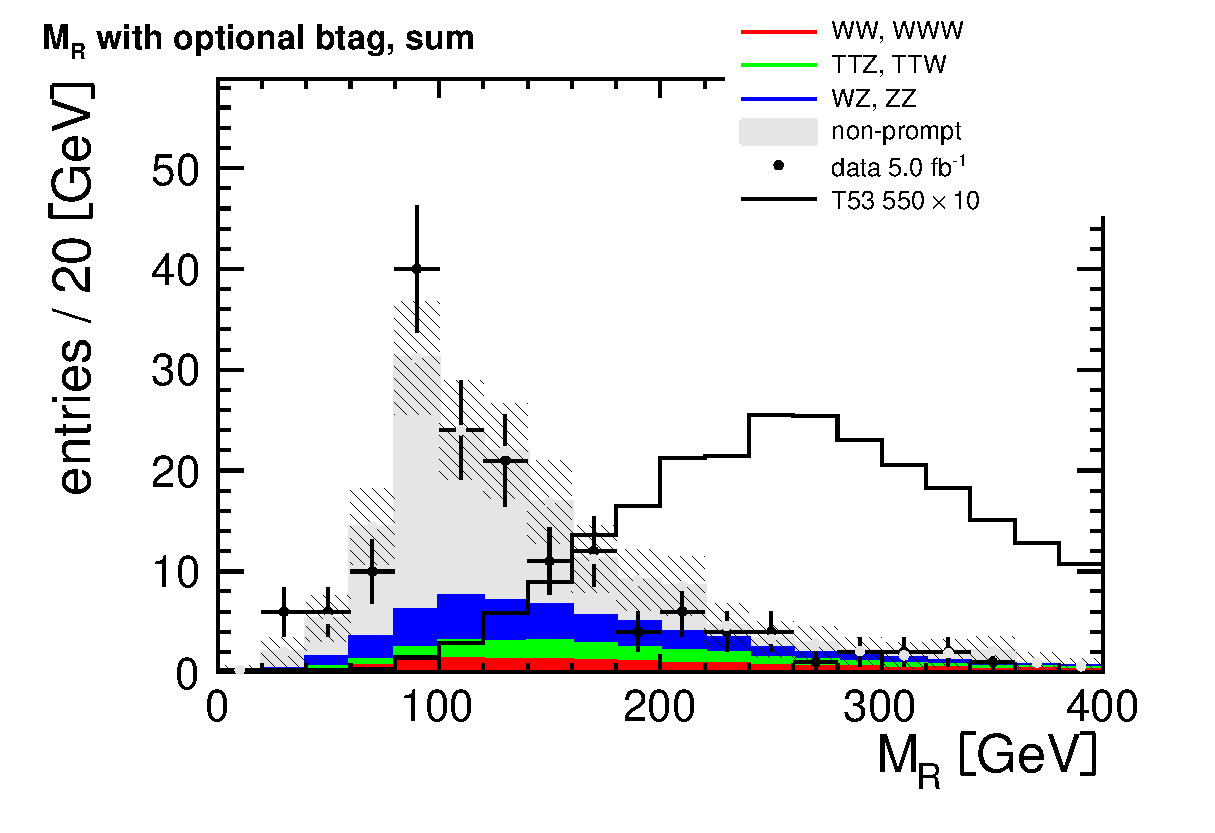
\includegraphics[width=.7\textwidth]{mr_optional_btag_sum.eps}
        \end{figure}
\end{frame}

\begin{frame}
    \frametitle{$R$}
    \framesubtitle{A dimensionless variable related to the \met}
    Theory:
    \begin{itemize}
        \item peaks near 0.5 for signal
        \item falls of exponentially for backgrounds after an endpoint
    \end{itemize}
        \begin{figure}[h]
            \centering
            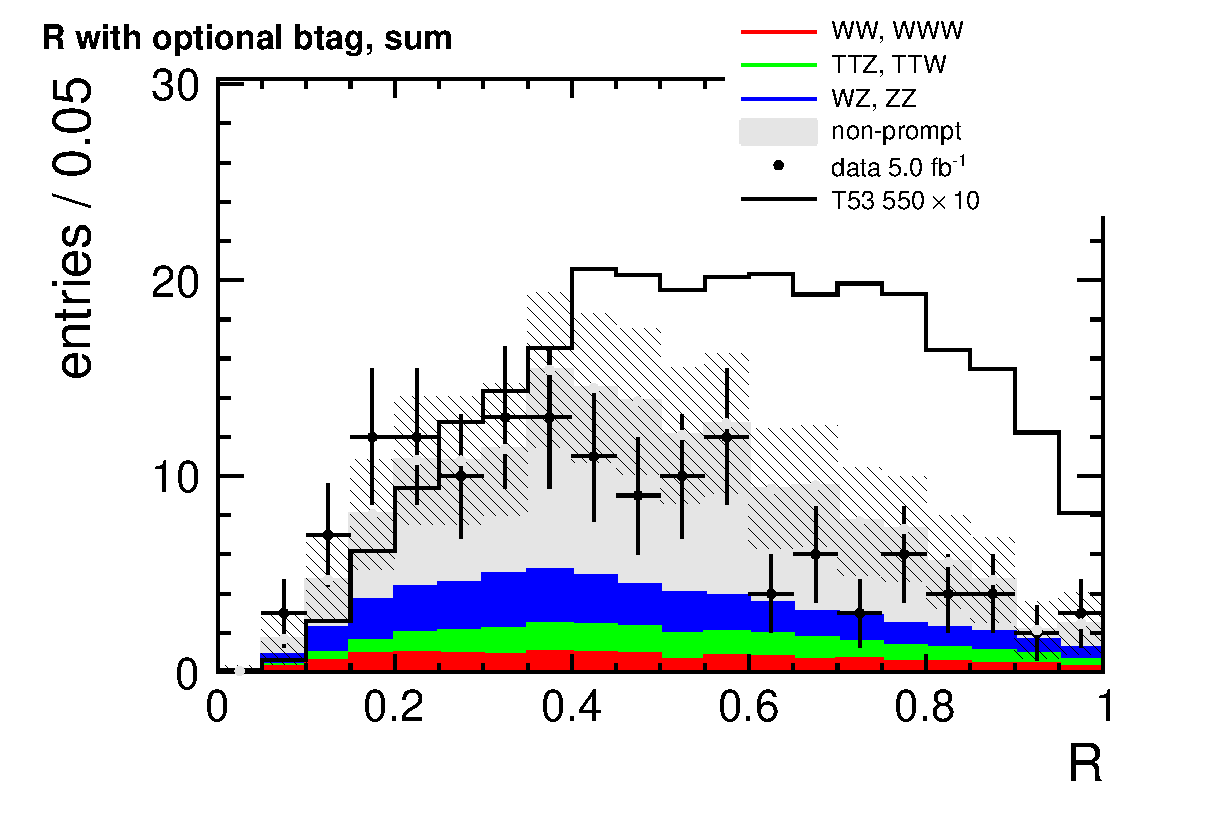
\includegraphics[width=.7\textwidth]{r_optional_btag_sum.eps}
        \end{figure}
\end{frame}

\begin{frame}
    \frametitle{Improving the variables}
    One of the b-jets belongs to the leptonic system: can we collect it?
    \begin{figure}[h]
        \centering
        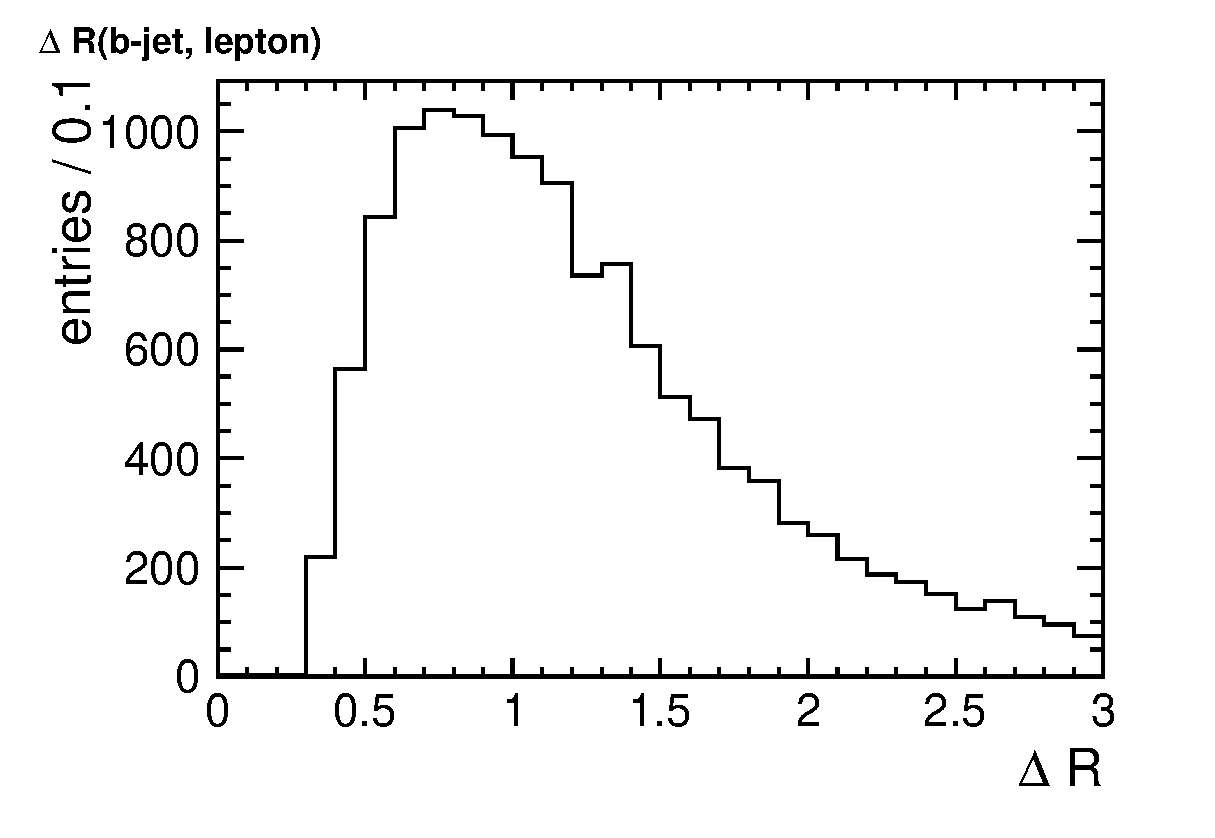
\includegraphics[height=.6\textheight]{signal_mc_dr_jet_lepton.eps}
        \caption{$\Delta R$ between the b-jet and the lepton from the top
            decay. MC truth from the \unit[550]{GeV} mass point.}
    \end{figure}
    MC suggests it should be the close to one of the leptons.
\end{frame}

\begin{frame}
    \frametitle{Event reconstruction enhancement and b-tagging}
    \begin{block}
        {Many jets and two leptons}
        The closest jet-lepton pair is the right one only in $1/3$ of the
        events.
    \end{block}

    \uncover<-2>{
        Improvements with b-tagging:
    \alert{If two b-tagged CSVL jets are found, the closest in $\Delta R$ to
    a lepton is associated with the lepton subsystem}

    \alert{MC truth: improves reconstruction for 1/2 of the signal events}
}
\end{frame}

\begin{frame}
    \frametitle{Improvements for the $M_R$}
    \framesubtitle{Without b-tagging}
        \begin{figure}[h!]
            \centering
                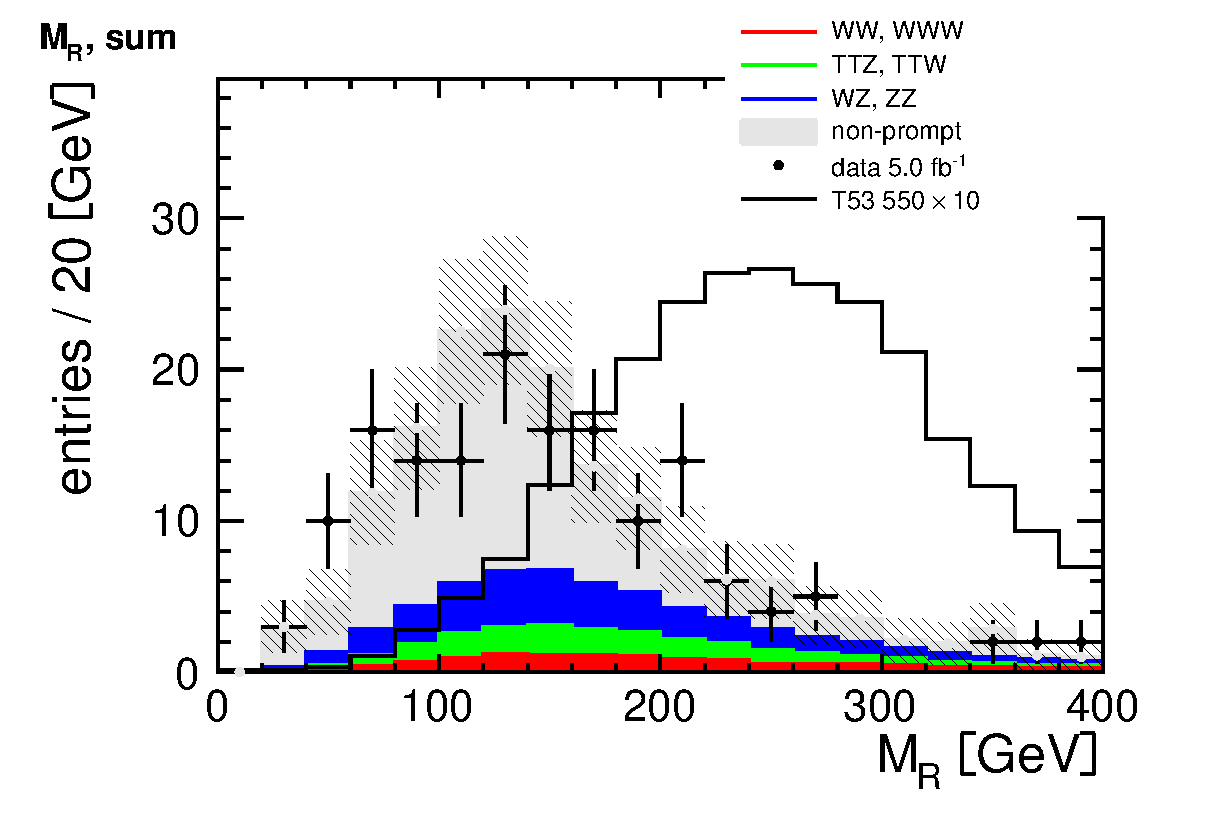
\includegraphics[height=.8\textheight]{mr_sum.eps}
        \end{figure}
\end{frame}

\begin{frame}
    \frametitle{Improvements for the $M_R$}
    \framesubtitle{With b-tagging}
        \begin{figure}[h!]
            \centering
                    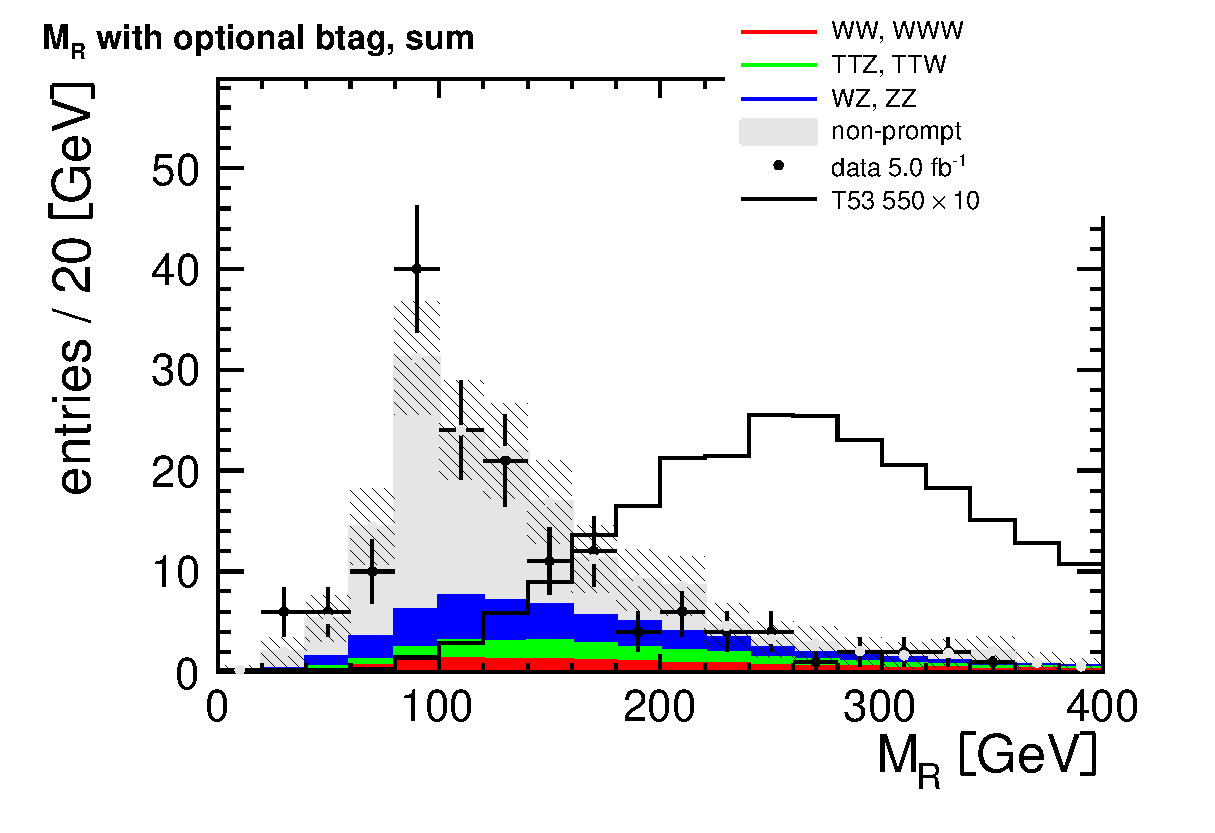
\includegraphics[height=.8\textheight]{mr_optional_btag_sum.eps}
        \end{figure}
\end{frame}

\begin{frame}
    \frametitle{Future improvements for the event reconstruction}
    \begin{itemize}
        \item the double b-tag is a tough requirement ($\varepsilon \approx 2/3$ on signal)
        \item wrong lepton close to a b-jet by chance ($\approx 1/3$)
        \item b-jet energy threshold
    \end{itemize}
\end{frame}

\begin{frame}
    \frametitle{Selection efficiencies for backgrounds}
    \framesubtitle{A better signal to noise ratio}
    Final razor selection optimized for $S/\sqrt{B}$. The current analysis
    requires two same-sign leptons, four jets, $H_T$. We are using the razor
    instead of $H_T$.
    \begin{itemize}
        \item hadronic mass $>\unit[350]{GeV}$
        \item $M_R > \unit[200]{GeV}$
        \item $R > 0.2$
    \end{itemize}
    \subimport{../../tables/}{background_efficiencies}
\end{frame}

\begin{frame}
    \frametitle{Selection efficiencies for signal}
    \framesubtitle{A better signal to noise ratio}
    \subimport{../../tables/}{signal_efficiencies}
\end{frame}

\begin{frame}
    \frametitle{Limit}
    \begin{description}
        \item[Expected:] \unit[658]{GeV} (it is \unit[645]{GeV} in AN-11-419)
    \end{description}
    \begin{figure}[h]
        \centering
    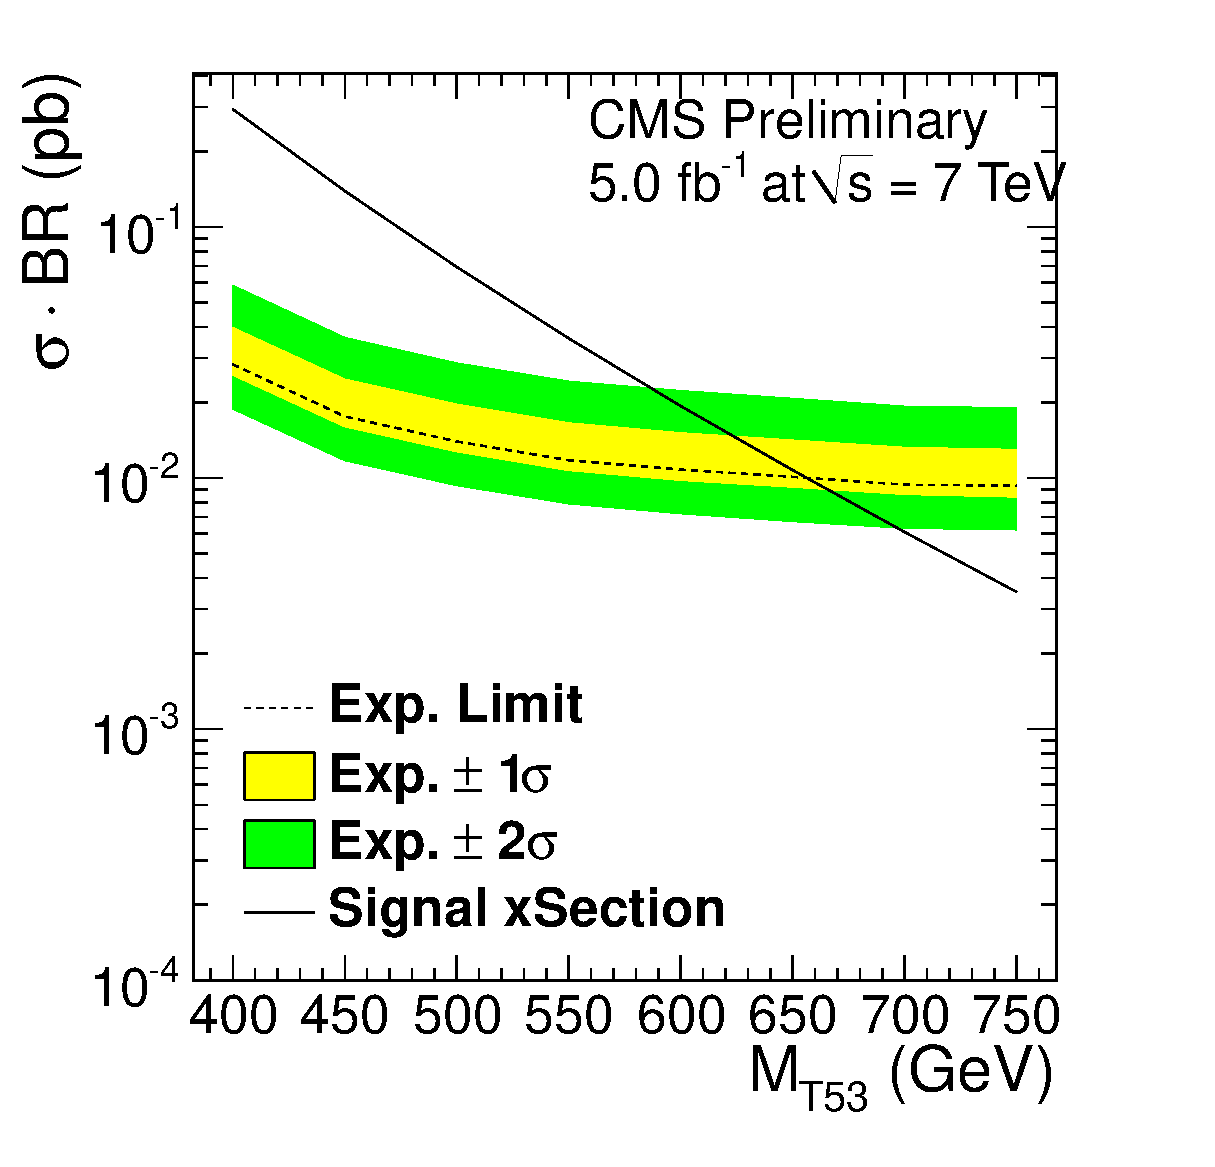
\includegraphics[height=.6\textheight]{oLimit_limit_macro_4jets_opt_btag_200_350_02.eps}
        \caption{95\% CL limit with the RooStats CL95 tool for an event
        counting experiment.}
    \end{figure}
\end{frame}

\begin{frame}
    \frametitle{Conclusions}
    \begin{itemize}
        \item much improved rejection of background, particularly $\ttbar$
        \item many areas for improvement in the event reconstruction
        \item need improved treatment of systematics
    \end{itemize}
\end{frame}

\begin{frame}
    \frametitle{Backup slides}
\end{frame}

\begin{frame}
    \frametitle{Systematics}
    \subimport{../../tables/}{systematics}
\end{frame}

\begin{frame}
    \frametitle{Systematics for MC}
    \subimport{../../tables/}{systematics_mc}
\end{frame}

\end{document}
